\let\negmedspace\undefined
\let\negthickspace\undefined
\documentclass[journal,12pt,onecolumn]{IEEEtran}
\usepackage{cite}
\usepackage{amsmath,amssymb,amsfonts,amsthm}
\usepackage{algorithmic}
\usepackage{graphicx}
\graphicspath{{Figs/}}
\usepackage{textcomp}
\usepackage{xcolor}
\usepackage{txfonts}
\usepackage{listings}
\usepackage{enumitem}
\usepackage{mathtools}
\usepackage{gensymb}
\usepackage{comment}
\usepackage{caption}
\usepackage[breaklinks=true]{hyperref}
\usepackage{tkz-euclide} 
\usepackage{listings}
\usepackage{gvv}                                        
%\def\inputGnumericTable{}                                 
\usepackage[latin1]{inputenc}     
\usepackage{xparse}
\usepackage{color}                                            
\usepackage{array}                                            
\usepackage{longtable}                                       
\usepackage{calc}                                             
\usepackage{multirow}
\usepackage{multicol}
\usepackage{hhline}                                           
\usepackage{ifthen}                                           
\usepackage{lscape}
\usepackage{tabularx}
\usepackage{array}
\usepackage{float}
%\newtheorem{theorem}{Theorem}[section]
%\newtheorem{theorem}{Theorem}[section]
%\newtheorem{problem}{Problem}
%\newtheorem{proposition}{Proposition}[section]
%\newtheorem{lemma}{Lemma}[section]
%\newtheorem{corollary}[theorem]{Corollary}
%\newtheorem{example}{Example}[section]
%\newtheorem{definition}[problem]{Definition}

\begin{document}


\title{4.3.58}
\author{AI25BTECH11002 - Ayush Sunil Labhade}
{\let\newpage\relax\maketitle}

\textbf{Question}:
		Show that the lines
		\begin{align}
\frac{x+3}{-3}=\frac{y-1}{1}=\frac{z-5}{5}
		\end{align}
		\begin{align}
		\frac{x+1}{-1}=\frac{y-2}{2}=\frac{z-5}{5}
		\end{align}
are coplanar.
	


\textbf{Solution:}

The given lines are
\begin{align}
L_1 &: \frac{x+3}{-3}=\frac{y-1}{1}=\frac{z-5}{5} \\
L_2 &: \frac{x+1}{-1}=\frac{y-2}{2}=\frac{z-5}{5}
\end{align}

In vector form:
\begin{align}
\vec{L_1} &= \myvec{-3 \\ 1 \\ 5}\lambda + \myvec{-3 \\ 1 \\ 5} \\
\vec{L_2} &= \myvec{-1 \\ 2 \\ 5}\mu + \myvec{-1 \\ 2 \\ 5}
\end{align}

So the direction vectors are
\begin{align}
\vec{m_1} = \myvec{-3 \\ 1 \\ 5} \quad 
\vec{m_2} = \myvec{-1 \\ 2 \\ 5}
\end{align}
and the vector between points on the two lines is
\begin{align}
\vec{B}-\vec{A} = \myvec{-1 \\ 2 \\ 5} - \myvec{-3 \\ 1 \\ 5} = \myvec{2 \\ 1 \\ 0}
\end{align}

For coplanarity, we check
\begin{align}
\rank \myvec{ \vec{m_1} & \vec{m_2} & \vec{B}-\vec{A} } \leq 2
\end{align}

That is,
\begin{align}
	\vec{M} = \myvec{ 
-3 & -1 & 2 \\
1 & 2 & 1 \\
5 & 5 & 0 
}.
\end{align}

Perform row reduction:

\begin{align}
\myvec{
-3 & -1 & 2 \\
1 & 2 & 1 \\
5 & 5 & 0
}
\xrightarrow[]{R_1 \leftrightarrow R_2}
\myvec{
1 & 2 & 1 \\
-3 & -1 & 2 \\
5 & 5 & 0
}
\end{align}

\begin{align}
\xrightarrow[]{R_2 \to R_2 + 3R_1,\; R_3 \to R_3 - 5R_1}
\myvec{
1 & 2 & 1 \\
0 & 5 & 5 \\
0 & -5 & -5
}
\end{align}

\begin{align}
\xrightarrow[]{R_3 \to R_3 + R_2}
\myvec{
1 & 2 & 1 \\
0 & 5 & 5 \\
0 & 0 & 0
}
\end{align}

Now the matrix is in echelon form.  

The rank of the matrix is \(2\).

$\therefore$ the given lines are coplanar.
		

Graph:
\begin{figure}[H]
    \centering
    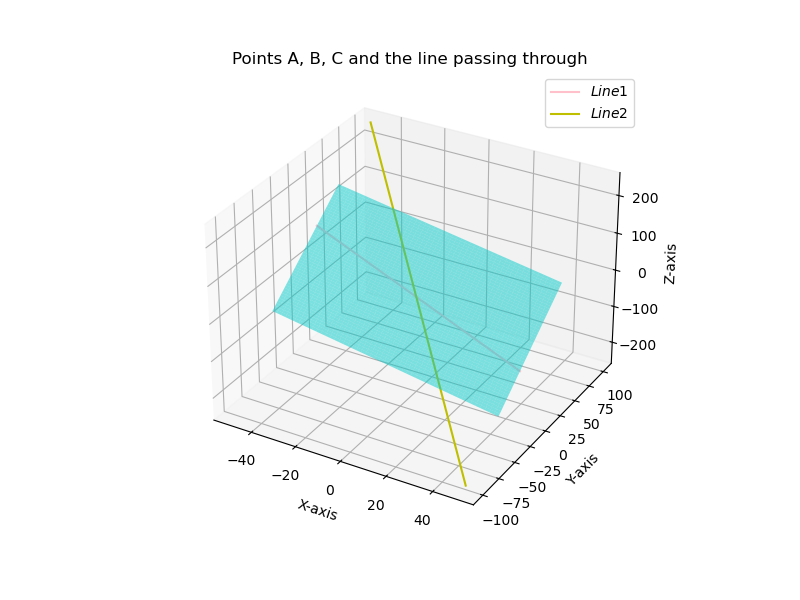
\includegraphics[scale=0.5]{plot}
    \caption{}
    \label{fig:plot}
\end{figure}
\end{document}
